%
% IEEE Transactions on Microwave Theory and Techniques example
% Tibault Reveyrand - http://www.microwave.fr
%
% http://www.microwave.fr/LaTeX.html
% ---------------------------------------



% ================================================
% Please HIGHLIGHT the new inputs such like this :
% Text :
%  \hl{comment}
% Aligned Eq. 
% \begin{shaded}
% \end{shaded}
% ================================================



\documentclass[journal]{IEEEtran}

%\usepackage[retainorgcmds]{IEEEtrantools}
%\usepackage{bibentry}  
\usepackage{multirow}
\usepackage[table,xcdraw]{xcolor}
\usepackage{xcolor,soul,framed} %,caption

\colorlet{shadecolor}{yellow}
% \usepackage{color,soul}
\usepackage[pdftex]{graphicx}
\graphicspath{{../pdf/}{../jpeg/}{../images/}}
\DeclareGraphicsExtensions{.pdf,.jpeg,.png}

\usepackage[cmex10]{amsmath}
%Mathabx do not work on ScribTex => Removed
%\usepackage{mathabx}
\usepackage{array}
\usepackage{mdwmath}
\usepackage{mdwtab}
\usepackage{eqparbox}
\usepackage{url}

\hyphenation{op-tical net-works semi-conduc-tor}

%\bstctlcite{IEEE:BSTcontrol}


%=== TITLE & AUTHORS ====================================================================
\begin{document}
\bstctlcite{IEEEexample:BSTcontrol}
    \title{Diseño y Simulación de un Reloj Digital con Circuitos Integrados}
  \author{Omar~Sanmartin,~\IEEEmembership{Student Member,~IEEE,}
      Ángel~Martinez,~\IEEEmembership{Student Member,~IEEE,}\\
      Johanna~Montaño,~\IEEEmembership{Student Member,~IEEE,}
      Miguel~Rojas,~\IEEEmembership{Student Member,~IEEE,}
      y~Cristian~Medina\'c,~\IEEEmembership{Student Member,~IEEE}% <-this % stops a space

  \thanks{Manuscript received July 10, 2012. \hl{This paper is an expanded paper from the IEEE MTT-S Int. Microwave Symposium held on June 17-22, 2012 in Montreal, Canada.} This work was funded in part by the Office of Naval Research under the Defense Advanced Research Projects Agency (DARPA) Microscale Power Conversion (MPC) Program under Grant N00014-11-1-0931, and in part by the Advanced Research Projects Agency-Energy (ARPA-E), U.S. Department of Energy, under Award Number DE-AR0000216.}
  \thanks{M. Roberg is with TriQuint Semiconductor, 500 West Renner Road Richardson, TX 75080 USA (e-mail: michael.roberg@tqs.com).}% <-this % stops a space
  \thanks{T. Reveyrand is with the XLIM Laboratory, UMR 7252, University of Limoges, 87060 Limoges, France (e-mail: tibault.reveyrand@xlim.fr).}%
  \thanks{I. Ramos and Z. Popovic are with the Department of Electrical, Computer and Energy Engineering, University of Colorado, Boulder, CO, 80309-0425 USA (e-mail: ignacio.ramos@colorado.edu; zoya.popovic@colorado.edu).}% <-this % stops a space
  \thanks{E. Falkenstein is with Qualcomm Inc., 6150 Lookout Road
Boulder, CO 80301 USA (e-mail: erez.falkenstein@gmail.com).}}  


% The paper headers
\markboth{IEEE TRANSACTIONS ON MICROWAVE THEORY AND TECHNIQUES, VOL.~60, NO.~12, DECEMBER~2012
}{Roberg \MakeLowercase{\textit{et al.}}: High-Efficiency Diode and Transistor Rectifiers}


% ====================================================================
\maketitle



% === ABSTRACT ====================================================================
% =================================================================================
\begin{abstract}
resumen
\end{abstract}


% === KEYWORDS ====================================================================
% =================================================================================
\begin{IEEEkeywords}
\hl{Key words}
\end{IEEEkeywords}

\IEEEpeerreviewmaketitle

% ========== I. INTRODUCTION =============
\section{Introduction}

\IEEEPARstart{T}{he} 
%=================================================================================
\section{Análisis para el diseño del Reloj Digital}
\subsection{Señal de reloj a través del temporizador 555.}
En la figura \ref{circuit_diagram} se muestra un generador de frecuencia de $1Hz$ utilizando el temporizador 555 el cual es cableado como un multivibrador Aestable.  Los pulsos de salida se pueden visualizar a través de un LED; este circuito no requiere ninguna señal externa para su funcionamiento.   Se puede calcular el valor de la frecuencia, utilizando la respectiva formula que se puede encontrar en el datasheet. Se tiene una frecuencia aproximada de $1Hz$.

% =======
% FIG. 01
% =======
\begin{figure}[h]
    \begin{center}
    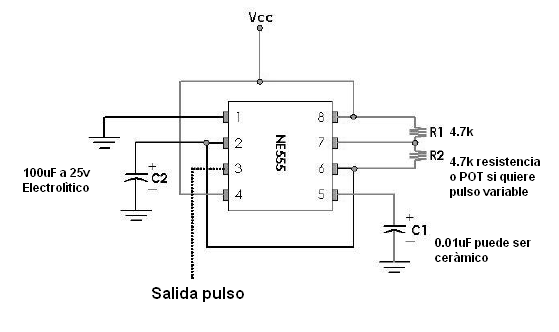
\includegraphics[width=8cm, height=5.5cm]{images/image1.png}
    \newline
    \caption{Circuito LM 555 de 1 segundo $\left ( 1Hz \right )$}\label{circuit_diagram}
    \end{center}
\end{figure}

\[\begin{array}{crl}
    f=\frac{1.44}{\left ( R_{1}+2R_{2}C_{1} \right )}
    \\
    \frac{1.44}{\left ( 10k+20k \right ) 47uF}
    \\
    \frac{1.44}{\left ( 30k \right ) 47uF}
    \\
    \frac{1.44}{1.41}=1.02Hz   
\end{array}\]
El intervalo de tiempo en que la salida está a nivel ALTO se define según:
\[\begin{array}{crl}
    t_{H}=0.7\left ( R_{1}+R_{2} \right )C_{1}
    \\
    0.7\left (10k+10k \right )47uF
    \\
    0.7\left ( 20k \right )47uF=0.658 seg
\end{array}\]
El intervalo de tiempo en que la salida está a nivel BAJO se define según: 
\[\begin{array}{crl}
    t_{L}=0.7R_{2}C_{1}
    \\ 
    0.7\left ( 10k \right )47uF=0.329 seg
\end{array}\]
El periodo $T$, de la señal de salida es la suma de $t_{H}$   y  $t_{L}$.  Esto es el reciproco de la frecuencia:
\[\begin{array}{crl}
    T=t_{H}+t_{L}
    \\
    0.658seg+0.329seg=0.987seg
\end{array}\]
Finalmente, el ciclo de trabajo es:
\[\begin{array}{crl}
    Ciclo~de~trabajo=\frac{t_{H}}{T}
    \\
    \frac{t_{H}}{t_{H}+t_{L}}
    \\
    \frac{0.658seg}{0.658seg+0.329seg}
    \\
    0.667*100\%=66.67\%
\end{array}\]
Una vez realizados los cálculos de frecuencia, periodo y ciclo de trabajo; se implementa el circuito en el simulador PROTEUS y a través de la utilización de un osciloscopio se puede observar la señal de salida del  temporizador, que se presenta como una señal no ideal debido al efecto de carga y descarga de los capacitores; pero que se puede utilizar como señal de reloj debido a que si es posible diferencia los flancos de subida y de bajada de cada uno de los pulsos.
Se debe notar adicionalmente que el ciclo de trabajo es del $66.67\%$, sin embargo esto no representara  inconvenientes  en  el  funcionamiento  del  reloj  digital,  ya  que  el  tiempo  o periodo  entre  las  transiciones  positivas  o  negativas  siempre  será  de  1  segundo aproximadamente $\left ( 0.987 \right )$, como se puede evidenciar en la figura \ref{osiloscop_sim}
\begin{figure}[h]
    \begin{center}
    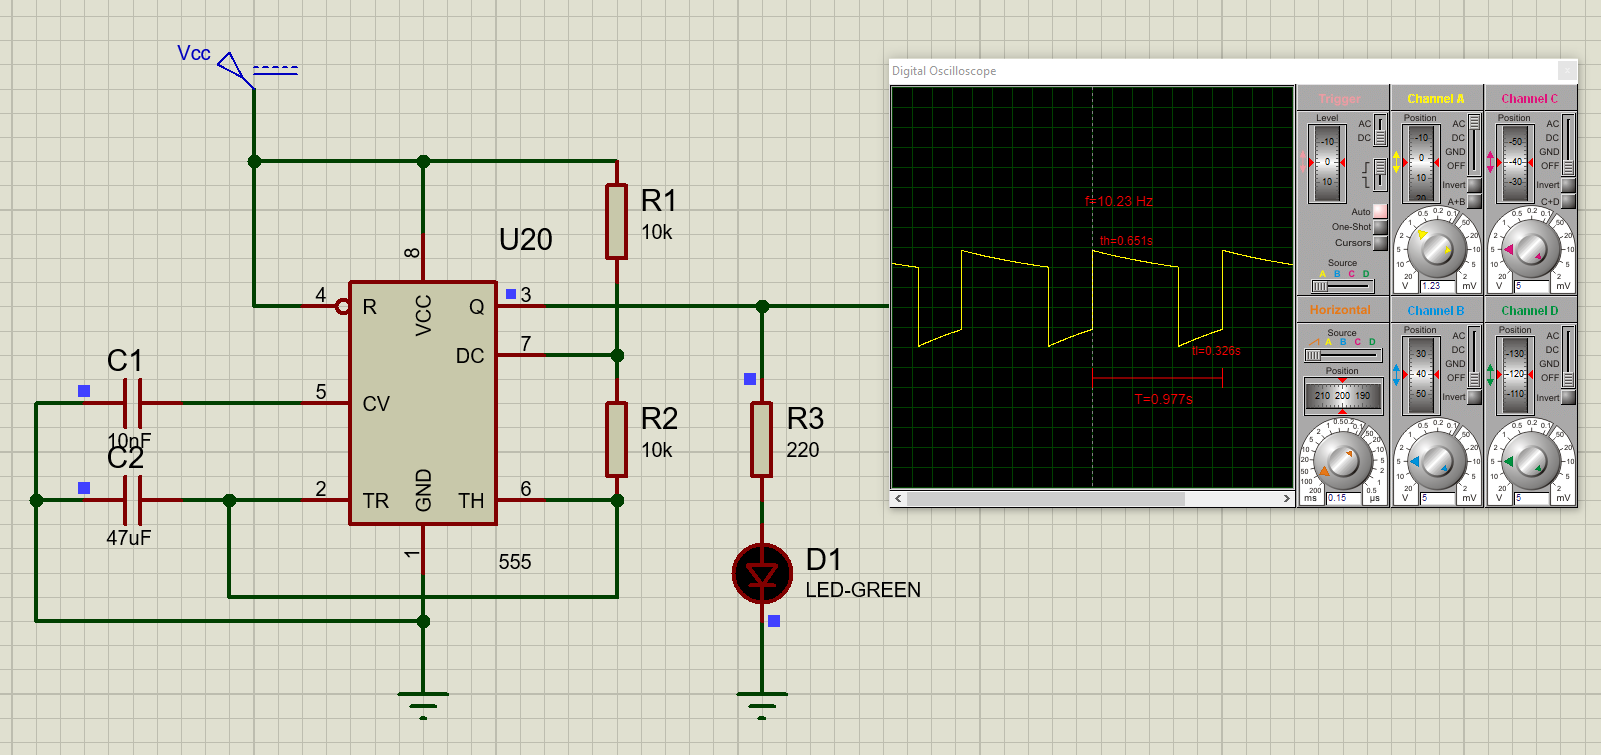
\includegraphics[width=8cm]{images/image3.png}
    \newline
    \caption{Datasheet 74ls90: Logic Diagram/Connection Diagram}\label{osiloscop_sim}
    \end{center}
\end{figure}

\subsection{Contador MOD10 y MOD6}
Para contador base que se utiliza para realizar el reloj digital de 24 horas es el 74LS90 que puede ser configurado como: MOD2, MOD3, MOD4, MOD5, MOD6, MOD7, MOD8, MOD9 y MOD10.
\begin{figure}[h]
    \begin{center}
    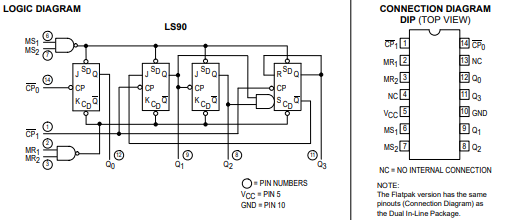
\includegraphics[width=8cm]{images/image2.png}
    \newline
    \caption{Datasheet 74ls90: Logic Diagram/Connection Diagram}\label{datasheet_diagram}
    \end{center}
\end{figure}
El 74LS90 es un contador de décadas síncrono, cuya configuración como MOD10 se muestra en la figura \ref{cont_MOD10}.
\begin{figure}[h]
    \begin{center}
    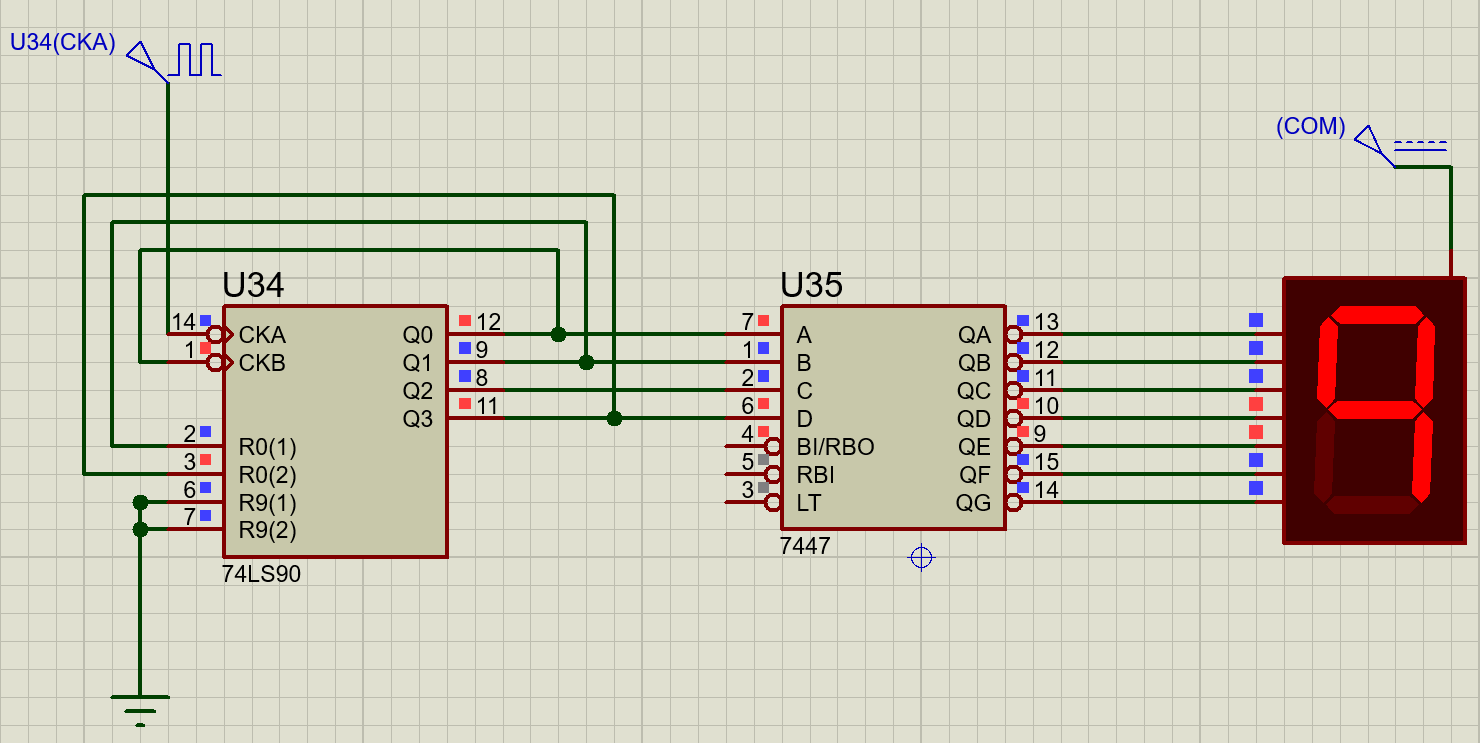
\includegraphics[width=8cm]{images/image4.png}
    \newline
    \caption{Contador MOD10 con 74LS90}\label{cont_MOD10}
    \end{center}
\end{figure}
Las  entradas  R0(1),  R0(2),  R9(1)  y  R9(2),  son  utilizadas  como  señales  de  PRESET  y CLEAR para cada uno de los Flip Flops del 74LS90; guiadas a través de dos compuertas NAND. En el datasheet estas entradas son etiquetadas como MS1, MS2, MR1 y MR2. 
\newline
El contador MOD6 se obtiene con la configuración de la Ilustración 5 donde las entradas R0(1) y R0(2) harán que las salidas de los Flip flops se hagan cero cuando se presente en la salida el valor binario 0110 y de esta forma el conteo solo sea desde cero hasta cinco.
\begin{figure}[h]
    \begin{center}
    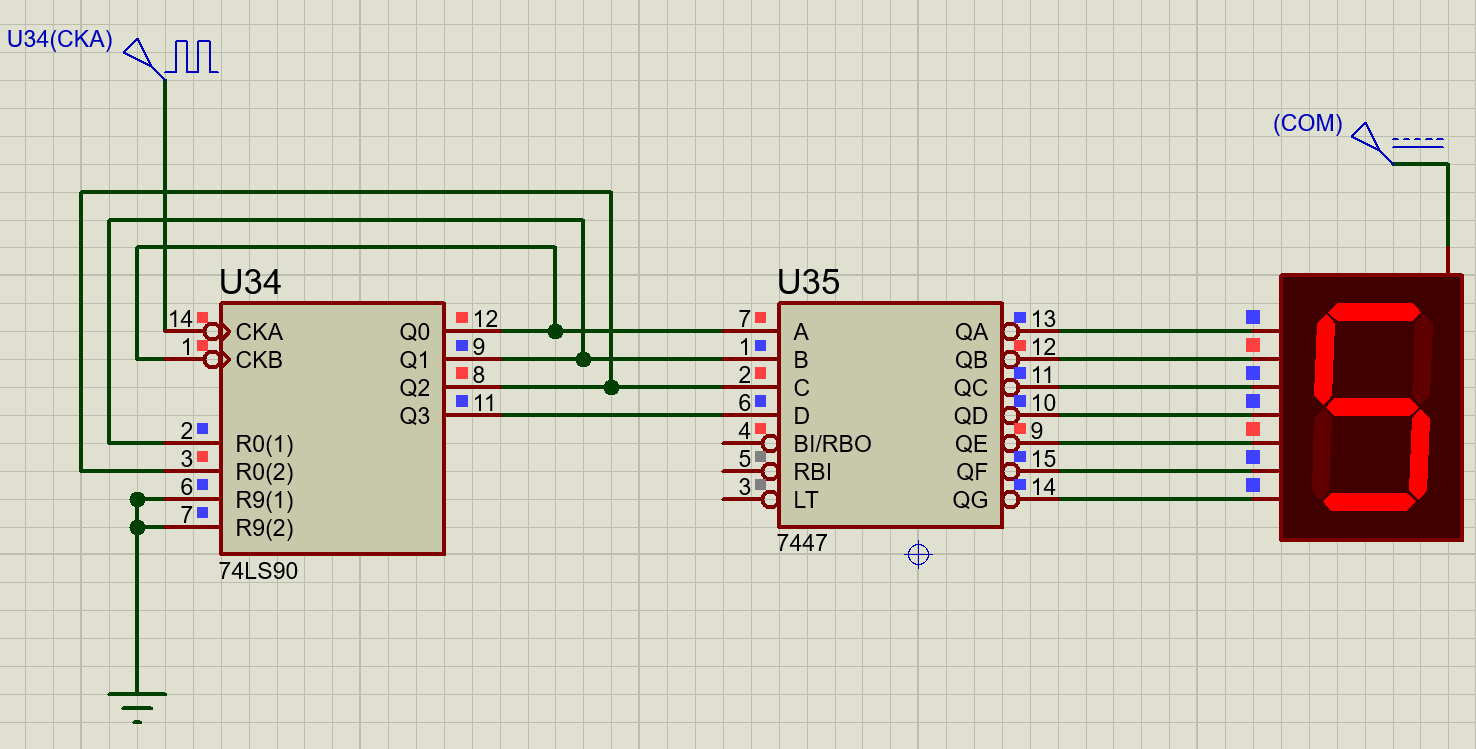
\includegraphics[width=8cm]{images/image5.png}
    \newline
    \caption{Contador MOD6 con 74LS90}\label{cont_MOD6}
    \end{center}
\end{figure}
\subsection{Diseño de reloj digital}
El diseño del reloj inicia con el conteo de los segundos, el cual tiene unidades y decenas. Las unidades de los segundos siempre tomaran valores entre 0 y 9; y cada vez que las unidades  tomen  el  valor  de  9  en  la  siguiente  transición  de  reloj  deberá  volver  a  0  y aumentar el contador de las decenas; es decir por cada vez que el contador MOD10 pase por sus 10 estados se deberá incrementar en uno el contador MOD6.  
\newline
Para conseguir esto de utiliza el bit más significativo del contador MOD10 como señal de reloj para el contador MOD6 y de esta forma obtener el conteo desde 00 hasta 59. 
\begin{figure}[h]
    \begin{center}
    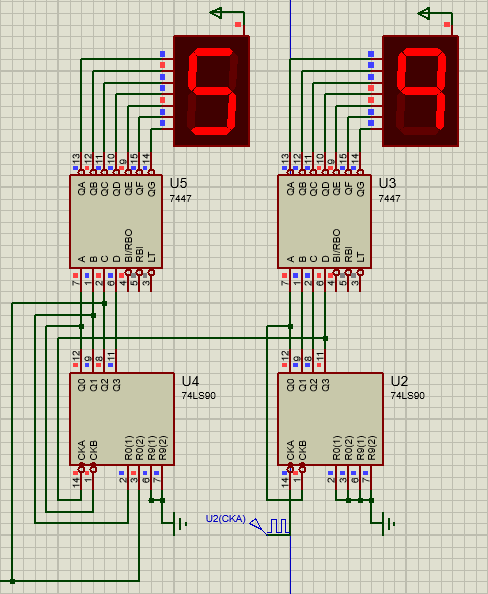
\includegraphics[width=8cm]{images/image6.png}
    \newline
    \caption{Contador de 00 a 59}\label{cont_59}
    \end{center}
\end{figure}
La lógica para realizar el conteo de los minutos es la misma, teniendo en consideración que cada vez que el segundero tome el valor de 59 en el siguiente ciclo de reloj los dos contadores de  los  segundos  deberán  volver  a  cero  y  el  contador  de  las  unidades de  los minutos deberá incrementar su valor.
\begin{figure}[h]
    \begin{center}
    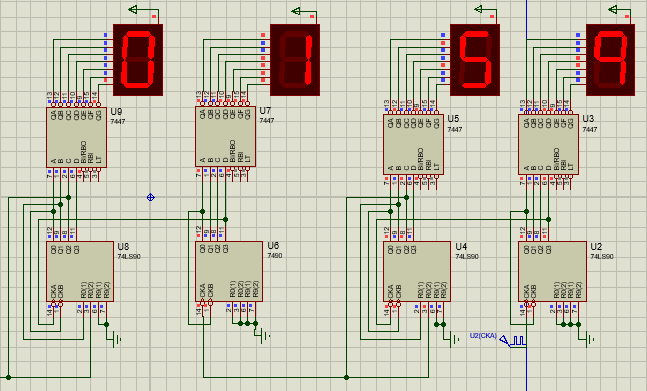
\includegraphics[width=8cm]{images/image7.png}
    \newline
    \caption{Contador segundos y minutos}\label{cont_hs}
    \end{center}
\end{figure}
Finalmente para contar las horas, se debe tener en cuenta que el reloj iniciará en 00 y terminará en 23; es decir el contador de las unidades y las decenas volverán a su estado inicial de 00 cuando se presente la condición que se muestra en la Tabla 1. A partir de esta condición que se presentará por un corto periodo de tiempo se reinician los contadores con el uso de una compuerta AND cuyas entradas serán:

\begin{figure}[h]
    \begin{center}
    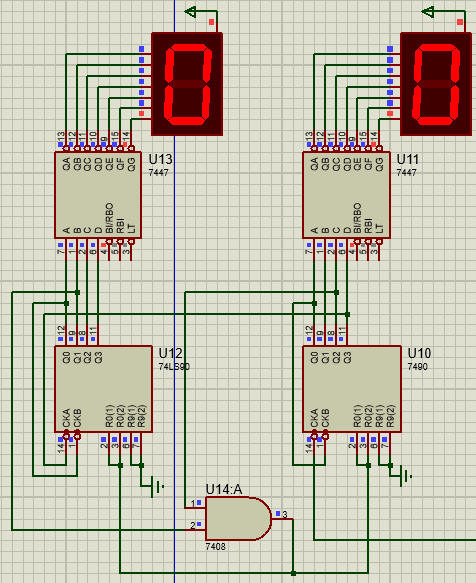
\includegraphics[width=8cm]{images/image8.png}
    \newline
    \caption{Contador de 24horas}\label{cont_24}
    \end{center}
\end{figure}
\begin{table}[]
    \begin{tabular}{|c|c|c|c|c|c|c|c|c|}
    \hline
    \multicolumn{9}{|c|}{CONTADOR DE HORAS} \\ \hline
    \multicolumn{4}{|c|}{CONTADOR DECENAS} & \multicolumn{4}{c|}{CONTADOR UNIDADES} &  \\ \cline{1-8}
    Q3 & Q2 & Q1 & Q0 & Q3 & Q2 & Q1 & Q0 & \multirow{-2}{*}{HORA} \\ \hline
    0 & 0 & 0 & 0 & 0 & 0 & 0 & 0 & 00 \\ \hline
    0 & 0 & 0 & 0 & 0 & 0 & 0 & 1 & 01 \\ \hline
    0 & 0 & 0 & 0 & 0 & 0 & 1 & 0 & 02 \\ \hline
    0 & 0 & 0 & 0 & 0 & 0 & 1 & 1 & 03 \\ \hline
    0 & 0 & 0 & 0 & 0 & 1 & 0 & 0 & 04 \\ \hline
    0 & 0 & 0 & 0 & 0 & 1 & 0 & 1 & 05 \\ \hline
    0 & 0 & 0 & 0 & 0 & 1 & 1 & 0 & 06 \\ \hline
    0 & 0 & 0 & 0 & 0 & 1 & 1 & 1 & 07 \\ \hline
    0 & 0 & 0 & 0 & 1 & 0 & 0 & 0 & 08 \\ \hline
    0 & 0 & 0 & 0 & 1 & 0 & 0 & 1 & 09 \\ \hline
    0 & 0 & 0 & 1 & 0 & 0 & 1 & 0 & 10 \\ \hline
    0 & 0 & 0 & 1 & 0 & 0 & 1 & 1 & 11 \\ \hline
    0 & 0 & 0 & 1 & 0 & 0 & 0 & 0 & 12 \\ \hline
    0 & 0 & 0 & 1 & 0 & 0 & 0 & 1 & 13 \\ \hline
    0 & 0 & 0 & 1 & 0 & 1 & 1 & 0 & 14 \\ \hline
    0 & 0 & 0 & 1 & 0 & 1 & 1 & 1 & 15 \\ \hline
    0 & 0 & 0 & 1 & 0 & 1 & 0 & 0 & 16 \\ \hline
    0 & 0 & 0 & 1 & 0 & 1 & 0 & 1 & 17 \\ \hline
    0 & 0 & 0 & 1 & 1 & 0 & 1 & 0 & 18 \\ \hline
    0 & 0 & 0 & 1 & 1 & 0 & 1 & 1 & 19 \\ \hline
    0 & 0 & 1 & 0 & 0 & 0 & 0 & 0 & 20 \\ \hline
    0 & 0 & 1 & 0 & 0 & 0 & 0 & 1 & 21 \\ \hline
    0 & 0 & 1 & 0 & 0 & 0 & 1 & 0 & 22 \\ \hline
    0 & 0 & 1 & 0 & 0 & 0 & 1 & 1 & 23 \\ \hline
    \rowcolor[HTML]{F8FF00} 
    0 & 0 & 1 & 0 & 0 & 1 & 0 & 0 & 24 \\ \hline
    0 & 0 & 0 & 0 & 0 & 0 & 0 & 0 & 00 \\ \hline
    0 & 0 & 0 & 0 & 0 & 0 & 0 & 1 & 01 \\ \hline
    0 & 0 & 0 & 0 & 0 & 0 & 1 & 0 & 02 \\ \hline
    \textbf{.} & \textbf{.} & \textbf{.} & \textbf{.} & \textbf{.} & \textbf{.} & \textbf{.} & \textbf{.} & \textbf{.} \\ \hline
    \textbf{.} & \textbf{.} & \textbf{.} & \textbf{.} & \textbf{.} & \textbf{.} & \textbf{.} & \textbf{.} & \textbf{.} \\ \hline
    \end{tabular}
    \caption{Tabla de Verdad de salida de contador de horas}\label{osiloscop_sim}
    \end{table}

    \begin{figure}[h]
        \begin{center}
        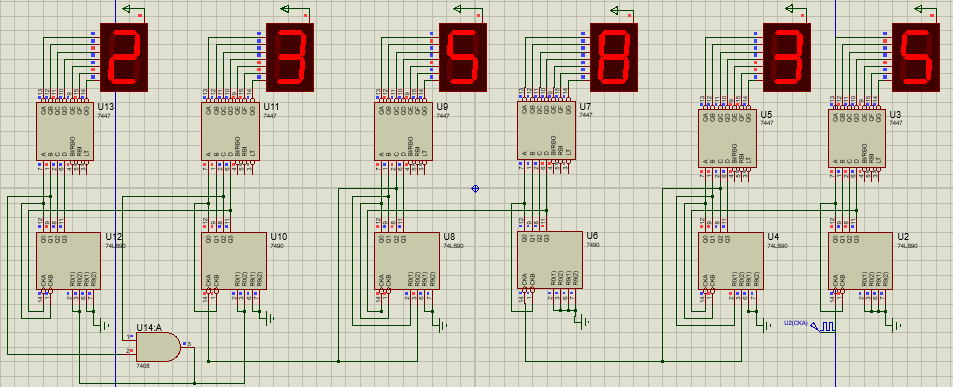
\includegraphics[width=8cm]{images/image9.png}
        \newline
        \caption{Diseño Final de Reloj Digital}\label{Diseño_final}
        \end{center}
    \end{figure}
\section{Conclusion}


\section*{Acknowledgment}


%Dr. Reveryrand would like to acknowledge the funding by XLIM, Limoges, France. 
The authors would like to thank Dr. David Root and Dr. Jean-Pierre Teyssier at Agilent Technologies for the loan of the time-domain nonlinear measurement equipment and TriQuint Semiconductor for the donation of the transistors. 



% if have a single appendix:
%\appendix[Proof of the Zonklar Equations]
% or
%\appendix  % for no appendix heading
% do not use \section anymore after \appendix, only \section*
% is possibly needed

% use appendices with more than one appendix
% then use \section to start each appendix
% you must declare a \section before using any
% \subsection or using \label (\appendices by itself
% starts a section numbered zero.)
%

% ============================================
%\appendices
%\section{Proof of the First Zonklar Equation}
%Appendix one text goes here %\cite{Roberg2010}.

% you can choose not to have a title for an appendix
% if you want by leaving the argument blank
%\section{}
%Appendix two text goes here.


% use section* for acknowledgement
%\section*{Acknowledgment}


%The authors would like to thank D. Root for the loan of the SWAP. The SWAP that can ONLY be usefull in Boulder...


% Can use something like this to put references on a page
% by themselves when using endfloat and the captionsoff option.
\ifCLASSOPTIONcaptionsoff
  \newpage
\fi



% trigger a \newpage just before the given reference
% number - used to balance the columns on the last page
% adjust value as needed - may need to be readjusted if
% the document is modified later
%\IEEEtriggeratref{8}
% The "triggered" command can be changed if desired:
%\IEEEtriggercmd{\enlargethispage{-5in}}

% ====== REFERENCE SECTION

%\begin{thebibliography}{1}

% IEEEabrv,

\bibliographystyle{IEEEtran}
% \bibliography{IEEEabrv,Bibliography}
%\end{thebibliography}
% biography section
% 
% If you have an EPS/PDF photo (graphicx package needed) extra braces are
% needed around the contents of the optional argument to biography to prevent
% the LaTeX parser from getting confused when it sees the complicated
% \includegraphics command within an optional argument. (You could create
% your own custom macro containing the \includegraphics command to make things
% simpler here.)
%\begin{biography}[{\includegraphics[width=1in,height=1.25in,clip,keepaspectratio]{mshell}}]{Michael Shell}
% or if you just want to reserve a space for a photo:

% ==== SWITCH OFF the BIO for submission
% ==== SWITCH OFF the BIO for submission





% \begin{IEEEbiography}[{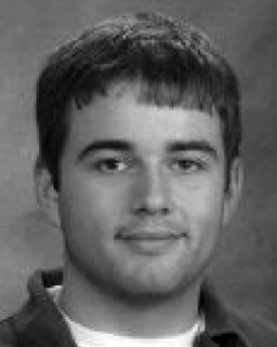
\includegraphics[width=1in,height=1.25in,clip,keepaspectratio]{photo/mike.png}}]{Michael Roberg}
% (S'09) received the B.S.E.E degree from Bucknell University, Lewisburg, PA, in 2003, the M.S.E.E. degree from the University of Pennsylvania, Philadelphia, in 2006, and the Ph.D. degree from the University of Colorado at Boulder in 2012. From 2003 to 2009, he was an Engineer with Lockheed Martin–MS2, Moorestown, NJ, where he was involved with advanced phased-array radar systems. His current research interests include high efficiency microwave PA theory and design, microwave power rectifiers, MMIC design, and high-efficiency radar and communication system transmitters. He is currently employed by TriQuint Semiconductor - Defense Products and Foundry Services in Richardson, TX working on wideband high efficiency GaN MMIC PA design.
% \end{IEEEbiography}
% \begin{IEEEbiography}[{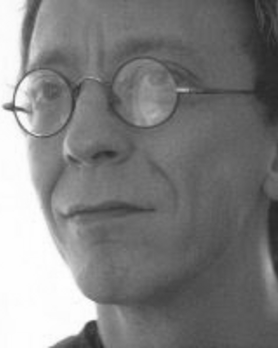
\includegraphics[width=1in,height=1.25in,clip,keepaspectratio]{photo/tibo.png}}]{Tibault Reveyrand}
% (M'07)  received the Ph.D. degree from the University of Limoges, France, in 2002.
% From 2002 to 2004, he was a Post-Doctoral Scientist with CNES (French Space Agency). In 2005, he became a CNRS engineer at XLIM. His research interests include the characterization and modeling of RF and microwave nonlinear components and devices.
% Dr. Reveyrand was the recipient of the 2002 European GaAs Best Paper Award and is a member of the IEEE MTT-11 "Microwave Measurements" Technical Committee.
% \end{IEEEbiography}
% \begin{IEEEbiography}[{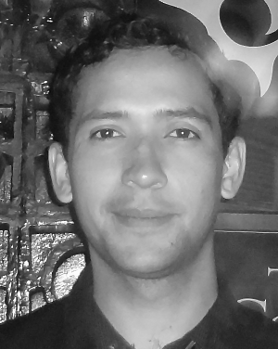
\includegraphics[width=1in,height=1.25in,clip,keepaspectratio]{photo/ignacio.png}}]{Ignacio Ramos}
% (S'12) received the B.S. degree in electrical engineering from the University of Illinois at Chicago in 2009, and is currently working toward the Ph.D. degree at the University of Colorado at Boulder. From 2009 to 2011, he was with the Power and Electronic Systems Department at Raytheon IDS, Sudbury, MA. His research interests include high-efficiency microwave power amplifiers, microwave DC/DC converters, radar systems, and wireless power transmission.
% \end{IEEEbiography}
% \begin{IEEEbiography}[{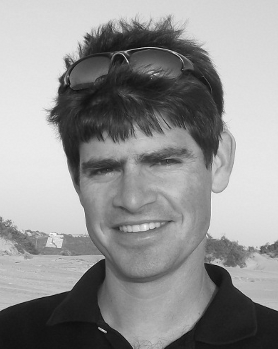
\includegraphics[width=1in,height=1.25in,clip,keepaspectratio]{photo/erez.png}}]{Erez Avigdor Falkenstein}
% (S'07), Haifa, Israel in 1979. He earned a “Handesaie” degree (associate degree) in electronics from Amal Handesaim School Hadera, Israel in 1999. From 1999 to 2003 he served in the Israel Defense Force as part of a technological unit. He has been at the University of Colorado at Boulder 2004 – 2012. He received concurrent MS/BS degrees in Electrical engineering 2010 and a Ph.D 2012 from the University of Colorado at Boulder. Since 2007 he has been involved with research as part of the active antenna group. Research emphasis: far field wireless powering for low power densities. Interests include Antenna design and characterization, modeling and measurement of nonlinear devices at microwave frequencies and power management. He is currently employed at Qualcomm, Incorporated, Boulder, CO.
% \end{IEEEbiography}
% \begin{IEEEbiography}[{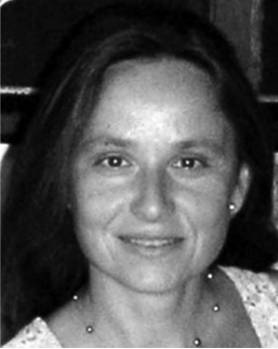
\includegraphics[width=1in,height=1.25in,clip,keepaspectratio]{photo/zoya.png}}]{Zoya Popovi\'c}
% (S'86-M'90-SM'99-F'02) received the Dipl.Ing. degree from the University of Belgrade, Belgrade, Serbia, Yugoslavia, in 1985, and the Ph.D. degree from the California Institute of Technology, Pasadena, in 1990.
% Since 1990, she has been with the University of Colorado at Boulder, where she is currently a Distinguished Professor and holds the Hudson Moore Jr. Chair with the Department of Electrical, Computer and Energy Engineering. In 2001, she was a Visiting Professor with the Technical University of Munich, Munich, Germany. 
% Since 1991, she has graduated 44 Ph.D. students. Her research interests include high-efficiency, low-noise, and broadband microwave and millimeter-wave circuits, quasi-optical millimeter-wave techniques, active
% antenna arrays, and wireless powering for batteryless sensors.
% Prof. Popovi\'c was the recipient of the 1993 and 2006 Microwave Prizes presented by the IEEE Microwave Theory and Techniques Society (IEEE MTT-S) for the best journal papers and the 1996 URSI Issac Koga Gold Medal. In 1997, Eta Kappa Nu students chose her as a Professor of the Year. She was the recipient of a 2000 Humboldt Research Award for Senior U.S. Scientists of the German Alexander von Humboldt Stiftung. She was elected a Foreign Member of the Serbian Academy of Sciences and Arts in 2006. She was also the recipient of the 2001 Hewlett-Packard (HP)/American Society for Engineering Education (ASEE) Terman Medal for combined teaching and research excellence.
% \end{IEEEbiography}





%% if you will not have a photo at all:
%\begin{IEEEbiographynophoto}{Ignacio Ramos}
%(S'12) received the B.S. degree in electrical engineering from the University of Illinois at Chicago in 2009, and is currently working toward the Ph.D. degree at the University of Colorado at Boulder. From 2009 to 2011, he was with the Power and Electronic Systems Department at Raytheon IDS, Sudbury, MA. His research interests include high-efficiency microwave power amplifiers, microwave DC/DC converters, radar systems, and wireless power transmission.
%\end{IEEEbiographynophoto}

%% insert where needed to balance the two columns on the last page with
%% biographies
%%\newpage

%\begin{IEEEbiographynophoto}{Jane Doe}
%Biography text here.
%\end{IEEEbiographynophoto}
% ==== SWITCH OFF the BIO for submission
% ==== SWITCH OFF the BIO for submission



% You can push biographies down or up by placing
% a \vfill before or after them. The appropriate
% use of \vfill depends on what kind of text is
% on the last page and whether or not the columns
% are being equalized.

\vfill

% Can be used to pull up biographies so that the bottom of the last one
% is flush with the other column.
%\enlargethispage{-5in}



% that's all folks
\end{document}